\chapter{Results and Discussion}
\label{chp:Results and Discussion}
This chapter documents the results from the trial conducted on the Ear-Monitor. The aim is to quantify the level of comparability between the measurements of the Ear-Monitor and the benchmark devices. Through this, an understanding of the accuracy of the Ear-Monitor will be obtained. Each participant is acting as his/her own control in this type of comparative analysis. Results are discussed one vital sign at a time.

\medskip

Correlation between each vital sign and its benchmark is visualised through an interclass correlation (ICC) plot. On each ICC plot, the $x=y$ line is plotted in black and a blue line is fitted to the data using the least squares method. Some of the terms used to evaluate correlation are defined as follows:

\begin{itemize}
\item Correlation coefficient (r): This quantifies the strength of the linear dependence between the values in the two datasets. r varies from -1 to 1. An correlation coefficient close to 1 indicates a high level of positive correlation between the Ear-Monitor and benchmark datasets and is a favourable result.

\item p-Value (p): The p-value is the probability of the data leading to an incorrect rejection of the null hypothesis, which is that there is no correlation between the Ear-Monitor and benchmark datasets. p-Values smaller than 0.05 indicate strong evidence against the null hypothesis, while p-values larger than 0.05 indicate weak evidence against the null hypothesis. $p=0$ indicates a p-value smaller than 0.00005, meaning that the correlation can be accepted with confidence.

\item ICC agreement (ICC\textsubscript{a}): This value ranges from 0 to 1 and the following, often quoted interpretation is suggested by \cite{cicchetti1994guidelines}:
\begin{itemize}
\item 0 to 0.40: Poor
\item 0.40 to 0.59: Fair
\item 0.60 to 0.74: Good
\item 0.75 to 1.00: Excellent
\end{itemize}

\item ICC consistency (ICC\textsubscript{c}): This quantifies the consistency of conclusions made by different observers. It ranges from 0 to 1, where values closer to 1 indicates higher consistency.

\item 95\% confidence intervals: These intervals are given for the ICC\textsubscript{a} and  ICC\textsubscript{c} values. If the interval should contain zero, then the ICC is not significant.
\end{itemize}

\section{Temperature Results}
The Ear-Monitor uses the TMP006 infrared sensor to measure the temperature of the tympanic membrane. The ET 100-A tympanic thermometer is used as the benchmark device. During each recording session, 15 Ear-Monitor and 3 ET 100-A data points are collected. It is assumed that the core temperature of the participant stays constant during the duration of the recording session. Therefore, the averages for the ET 100-A and Ear-Monitor measurements are compared. This is a valid assumption, for the standard deviations within recording sessions are found to be between 0.0018 and \SI{0.0814}{\celsius}. Datasets recorded from participants 1 and 5 are removed due to faulty recording sessions.

\medskip

Results from the two calibration approaches are documented separately and then compared in the discussion. The results for the two different calibration methods are summarised in Appendix \ref{Data Tables}. All participants are healthy and benchmark temperatures range from 36.33 to \SI{38.55}{\celsius}.

\subsection{Group Calibration Results}
Equation \ref{eq:TempCal} is used by the Ear-Monitor to calculate the tympanic temperature of participants. Figure \ref{fig:Temp1Scatter} depicts an ICC plot of the Ear-Monitor versus ET 100-A data points for the 28 recording sessions. The mean error is 0.0180 $\pm$\SI{0.5125}{\celsius}.

\begin{figure}[H]
   \centering
   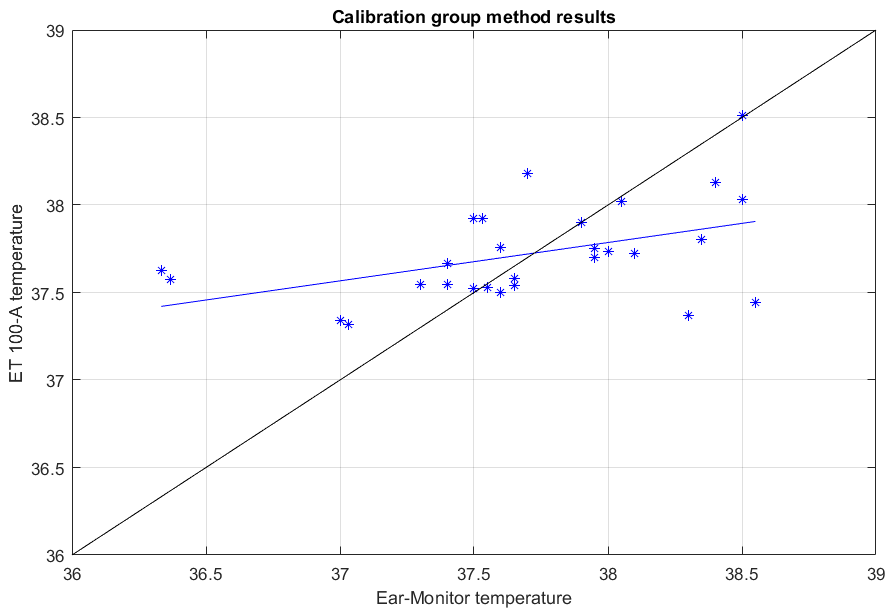
\includegraphics[width=13cm,height=8cm]{figs/Temp1Scatter.png}
   \caption{Temperature through the Group calibration method: ET 100-A vs. Ear-Monitor}
   \label{fig:Temp1Scatter}
\end{figure}

\subsection{Intra-participant Calibration Results}
This method uses data from the first recording session to calibrate the Ear-Monitor, and the data from the second session to evaluate the calibration. Figure \ref{fig:Temp2Scatter} depicts an ICC plot of the Ear-Monitor versus ET 100-A data points for the 14 recording sessions used for evaluation. The recording sessions used for calibration are not plotted, for they all lay on the $x=y$ line. The mean error is -0.0156 $\pm$\SI{0.29}{\celsius}.

\begin{figure}[H]
   \centering
   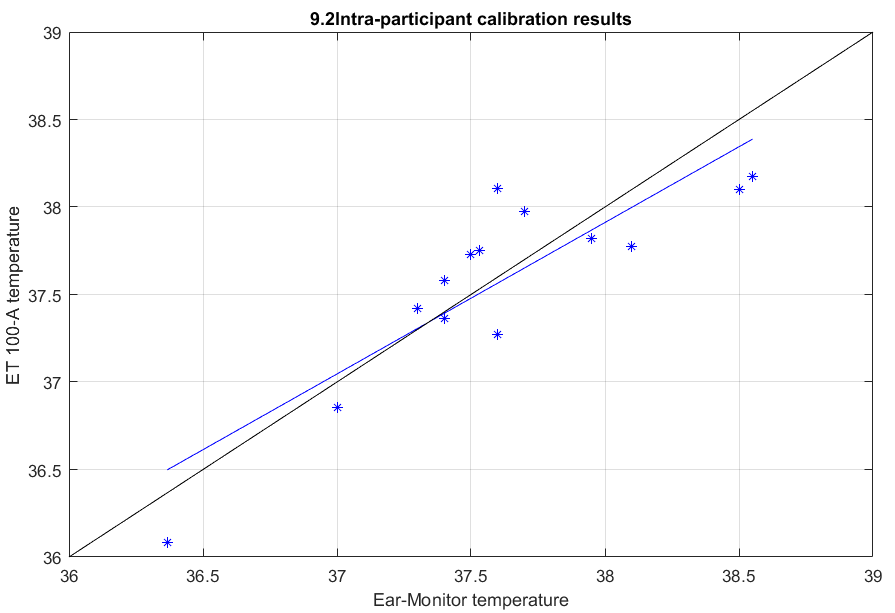
\includegraphics[width=13cm,height=8cm]{figs/Temp2Scatter.png}
   \caption{Temperature through the Intra-participant calibration method: ET 100-A vs. Ear-Monitor}
   \label{fig:Temp2Scatter}
\end{figure}

\medskip

\subsection{Temperature Results Discussion}
The measurements inside a recording session are close to one another, with a maximum standard deviation of \SI{0.0814}{\celsius}. This demonstrates the high precision of the TMP006, making it the right choice for an infrared sensor. This level of precision is owed to the thermal consistency inside the ear canal. Air flow is negligible and the position of objects in the sensor's field of vision stays constant.

\medskip

The two different calibration methods can be compared through a box and whisker plot of their respective errors, as depicted in Figure \ref{fig:ComparingCalibrationBoxplot}. The superiority of the intra-participant calibration method can be observed in the smaller first and fourth quartiles. This indicates a significant reduction in large errors.

\begin{figure}[H]
   \centering
   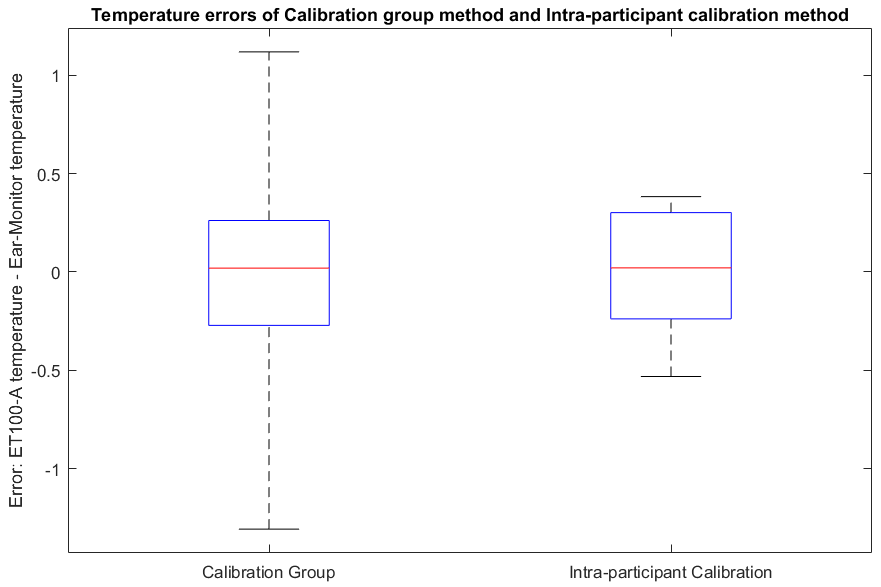
\includegraphics[width=12cm,height=7.5cm]{figs/ComparingCalibrationBoxplot.png}
   \caption{Temperature errors of the Group calibration and Intra-participant calibration methods}
   \label{fig:ComparingCalibrationBoxplot}
\end{figure}

The 95\% confidence intervals for ICC\textsubscript{a} and ICC\textsubscript{c} for the group calibration method includes zero, which means that the correlation is not significant. Whereas, the ICC intervals for the intra-participant calibration method is above zero, indicating good correlation. Furthermore, the p-value is far below 0.05, indicating a negligible probability of zero correlation. The data unanimously indicate that the intra-participant calibration method is superior to the group calibration method with regards to accuracy and correlation. 

\medskip

Although the intra-participant calibration method produces the best results, it should be kept in mind that this method requires a calibration sequences when it is used for the first time on an individual. The merit in the group calibration method lies in the fact that calibration is done only once, during manufacturing. With better probe design, the TMP006 can be located more consistently between different individuals and the group calibration method can become more accurate. But as it is now, the intra-participant calibration method is the preferred.

\medskip

As mentioned in the literature review, there are not many published results of wearable ear temperature monitors to compare the Ear-Monitor to. There are, however, commercial devices available for comparison. The Novatemp\textsuperscript{\textregistered{}} and Starboard\textsuperscript{\textregistered{}} both claims a standard accuracy of $\pm\SI{0.2}{\celsius}$ \citep{Novatemp, Starboard} and the Cosinuss Degree\textsuperscript{\textregistered{}}, a standard accuracy of $\pm\SI{0.1}{\celsius}$ \citep{CosinussDegree}. The Ear-Monitor with intra-participant calibration comes close to this, with a standard accuracy of $\pm$\SI{0.29}{\celsius}.

%---------------------------------------------------------------------------------------------------------------------------------------------

\section{Heart Rate Results}
The Ear-Monitor uses an infrared PPG obtained by the MAX30100 in the ear canal to detect heartbeats via a beat detection algorithm. The average period between 10 successive detected beats is used to calculate the heart rate. The beat detection algorithm is at the core of the heart rate functionality of the Ear-Monitor, and therefore it is evaluated independently. This is followed by comparative analysis between the individual beat periods and 10-beat moving average heart rates of the Ear-Monitor and Nexus-10 physiological monitor.

\subsection{Beat Detection Algorithm Evaluation Results}
The beat detection algorithm used by the Ear-Monitor is first tested on open source data from PhysioNet.org, and then on the data collected during the trial. The results of these two tests are discussed separately.

\subsubsection{PhysioNet Data Test}
The beat detection algorithm is tested on PPG data from the open-source MIMIC Database on PhysioNet.org \citep{PhysioNet}. This data was recorded from patients in intensive care units and is made available for developing and testing intelligent monitoring systems. PPG data is recorded with clinical finger pulse oximeters. Ten-minute segments from 14 different patients are used to test the algorithm. Each set of data also includes an ECG signal, which is used to identify the benchmark beats. The results for this test can be seen in Appendix \ref{Data Tables}.

\medskip

Of the 12001 beats in all the PhysioNet test datasets, 13 (0.108\%) false positives and 91 (0.758\%) false negatives are detected. Even though the beat detection algorithm is designed and tuned using PPGs collected from the ear canal wall, it can accurately detect beats from finger pulse oximeters. This result demonstrates the robustness of the algorithm. Most false detections occurred where signals were corrupted by noise. This result also demonstrates how the SSF can extract beats, even from a noisy signal.

\subsubsection{Trial Data Test}
Subsequently, the algorithm is tested using the data collected during the trial. The number of beats detected for each participant by the Ear-Monitor is compared to the number of benchmark beats. The supporting software for the Nexus-10, BioTrace+, has a peak detection algorithm, but it is found that it misses some peaks. To ensure accurate benchmark peak detection, the PPG from the Nexus-10 is inspected manually and peaks are marked by a human annotator. Figure \ref{fig:BeatDetectionTest} depicts plots of (a) the Ear-Monitor SSF with detected beats and (b) the Nexus-10 PPG signal with annotated beats. In this example, 100\% of the peaks are detected by Ear-Monitor.

\begin{figure}[H]
\centering
\graphicspath{{figs/}}
\input{figs/BeatDetectionTest.pdf_tex}
\caption{Plots of (a) the Ear-Monitor SSF with detected beats and (b) the Nexus-10 PPG signal with annotated beats} %Marga1_Data
\label{fig:BeatDetectionTest}
\end{figure}

Appendix \ref{Data Tables} tabulates the results of the beat detection evaluation. Of the 4713 beats in the participant trial data, 10 (0.21\%) false positives and 58 (1.23\%) false negatives are detected. The mean error of the sample group is -1.5313 $\pm$2.8847 beats. It should also be noted 51 of the false negatives (87.9\%) are from the data collected from three of the participants: 5, 9 and 13.

\medskip

Figure \ref{fig:BeatDetectionScatter} depicts an ICC plot of the number of annotated Nexus-10 beats versus the number of detected Ear-Monitor beats. Data recording sessions from all 16 trial participants are used, which means 32 sets of data points are compared.

\begin{figure}[H]
   \centering
   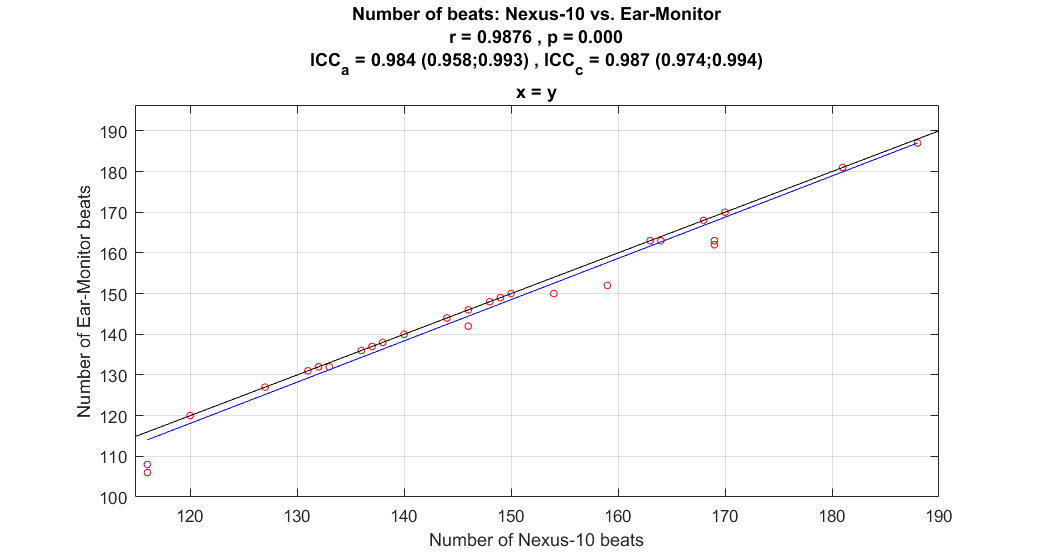
\includegraphics[width=12cm,height=7.5cm]{figs/BeatDetectionScatter.png}
   \caption{Number of beats: Nexus-10 vs. Ear-Monitor}
   \label{fig:BeatDetectionScatter}
\end{figure}

This test demonstrates that the Ear-Monitor performs well in its task of detection beats. The number of false negatives detected for the trial data is higher than for the PhysioNet data. This can be ascribed to the fact that the PPG from three of the participants was of a notably lower quality. Although the adaptive threshold method detected the majority of the peaks, the amplitude of the SSF peaks varied prominently and very low amplitudes were missed by the algorithm. This can be caused by low blood profusion in the ear canal or bad contact between the MAX30100 and the canal wall.

\subsection{Beat Period and Average Heart Rate Results}
The accuracy of the heartbeat period is tested to determine if beats are detected at the right position in time. Periods between subsequent  beats detected by the Ear-Monitor are compared to periods between beats annotated on the Nexus-10 PPG. Figure \ref{fig:PeriodScatter} depicts an ICC plot of Nexus-10 versus Ear-Monitor periods. A total of 4569 periods from the 16 participants is compared. Benchmark periods ranged from 575.65 to \SI{1198}{\milli\second}. The mean error of the sample group is 0.0821 $\pm$\SI{50.71}{\milli\second}.

\begin{figure}[H]
   \centering
   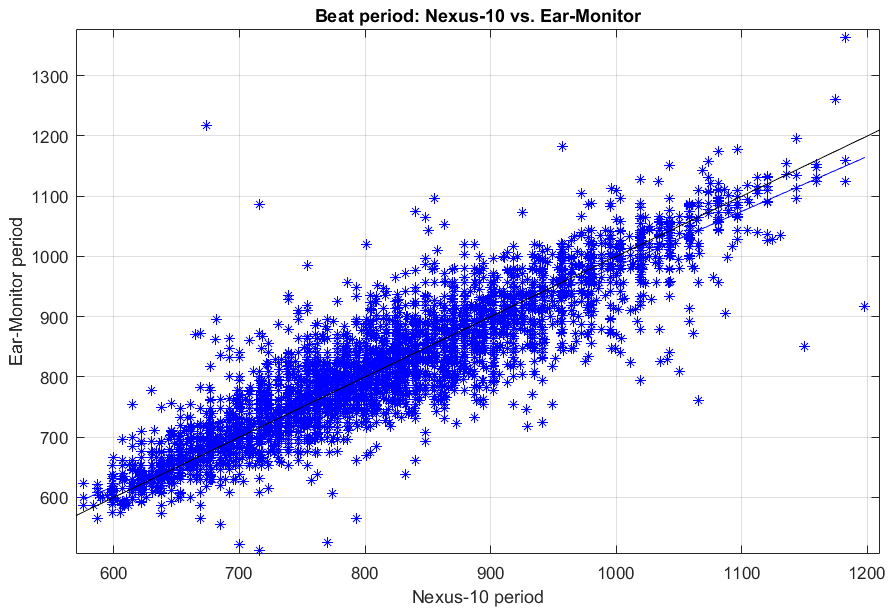
\includegraphics[width=12cm,height=7.5cm]{figs/PeriodScatter.png}
   \caption{Beat period: Nexus-10 vs. Ear-Monitor}
   \label{fig:PeriodScatter}
\end{figure}

The 10-beat average heart rate is calculated from the Ear-Monitor and Nexus-10 data and compared in the same way as with the beat periods. Figure \ref{fig:HeartRateScatter} depicts an ICC plot of Nexus-10 versus Ear-Monitor heart rates. A total of 4258 periods are compared from 16 participants with benchmark heart rates varying from 54.2 to 100.0 bpm. The mean error of the sample group is 0.0306 $\pm$0.7174 bpm.

\begin{figure}[H]
   \centering
   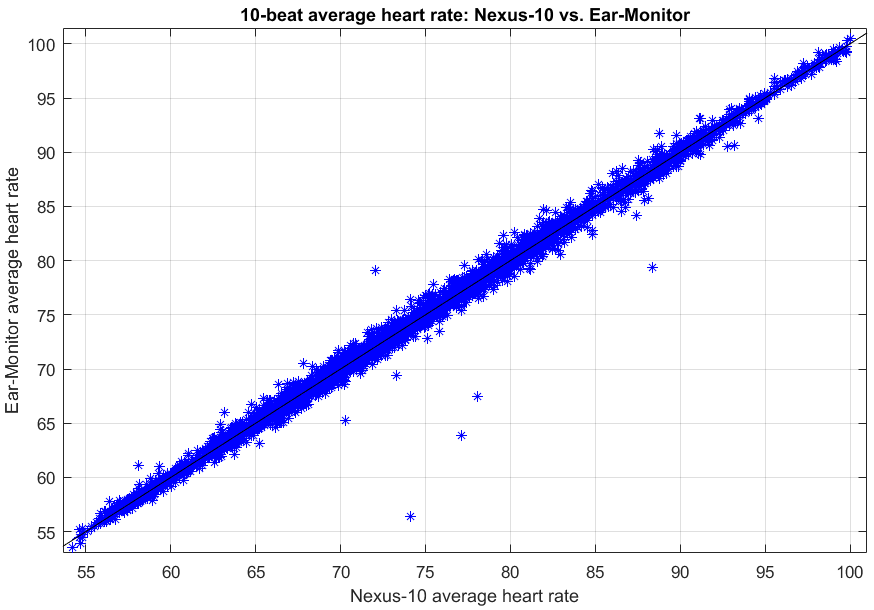
\includegraphics[width=12cm,height=7.5cm]{figs/HeartRateScatter.png}
   \caption{10-beat average heart rate: Nexus-10 vs. Ear-Monitor}
   \label{fig:HeartRateScatter}
\end{figure}

\subsection{Heart Rate Results Discussion}
The beat detection algorithm is evaluated based on PhysioNet data and data collected from participants during the trial. The algorithm performed better on the PhysioNet data than on the trial data. This can be ascribed to the fact that three of the participants contributed to 87.9\% of the false negatives detected in the trial data. These are all participants with smaller external ears, which is emphasized by the fact that two of them are female. This highlights the effect the fit of the ear probe in the ear has on the accuracy of the beat detection algorithm. A bad fit causes non-ideal contact between the MAX30100 and the canal wall, as well as reducing subcutaneous blood perfusion.  This is a patient specific inaccuracy and can be overcome by a more customised ear probe.

\medskip

Even with these three individuals, the beat detection algorithm performs exceptionally good. On average 1.5313 $\pm$2.8847 beats are missed per 2-minute recording session. The correlation of the number of beats detected between the Ear-Monitor and the benchmark device is high, with a correlation coefficient of 0.9876 and a p-value of zero. The ICC\textsubscript{a} and ICC\textsubscript{c} are both excellent within a 95\% confidence interval.

\medskip

The beat period ICC plot in Figure \ref{fig:PeriodScatter} depicts a clear correlation. The large number of data points reveals the normal distribution of the data. The correlation coefficient, p-value, ICC\textsubscript{a} and ICC\textsubscript{c} all indicate an excellent correlation. The Ear-Monitor can measure the period between heartbeats with a mean error of 0.0821 $\pm$\SI{50.71}{\milli\second}. This notably high accuracy is improved even further by calculating the 10-beat average heart rate. The ICC plot of the average heart rate in Figure \ref{fig:HeartRateScatter} illustrates an exceptional correlation between the Ear-Monitor and benchmark measurements. The Ear-Monitor can measure the heart rate of participants with a mean error of 0.0306 $\pm$0.7174 bpm relating to a 1.04\% error at 72 bpm. This compares favourably to the commercial wrist worn heart rate monitors reviewed by \cite{shcherbina2017accuracy}.

%---------------------------------------------------------------------------------------------------------------------------------------------

\section{Respiratory Rate Results}
The Ear-Monitor uses respiratory sinus arrhythmia (RSA), the frequency modulating respiratory related heart rate characteristic, to extract a respiratory rate. The chest strap connected to the Nexus-10 physiological monitoring platform is used to measure the benchmark respiration rate. Benchmark breaths from the Nexus-10 are manually annotated. The recording session consisted of one minute of normal breathing followed by one minute of regulated breathing at 15 breaths per minute. Appendix \ref{Data Tables} tabulates the results of the breaths detected for the 16 participants. Benchmark respiratory rates of the participants varied from 7 to 28 breaths per minute. The mean error is 0.0156 $\pm$3.9081 breaths per minute.

\medskip
It should be noted, however, that the majority of the inaccuracies can be traced to the recording sessions of participants 5, 9 and 13. Upon closer inspection, the following explanation can be given. Participant 5 and 13 both have a large number of false positives, the highest and third highest average heart rates and very low heartbeat period variation due to RSA. Participant 9 has an unusually high resting respiratory rate (more than double that of the average of the rest of the participants), bordering on the maximum measurable rate according to the Nyquist theorem, which is equal to half the heart rate. This caused 51\% of breaths to be missed during normal breathing. As expected, when the respiratory rate was lowered during the controlled breathing exercise, the breath detection accuracy returned to the group average. These three participants are regarded as outliers and are isolated from the rest in order to reveal the trends present in the bulk of the recording sessions.

\medskip

The mean errors in respiratory rate between the benchmark Nexus-10 and the Ear-Monitor can be seen in Table \ref{tab:BreathingAccuracies}. Standard deviations are included and all values are in breaths per minute. When removing the outliers, the mean error of the normal and controlled breathing groups are closer to one another and the standard deviation of the errors are reduced by more than half.

\begin{table}[H]
\caption{Mean errors of the respiratory rate measurements}
\label{tab:BreathingAccuracies}
\renewcommand{\arraystretch}{1.2}
\centering
\begin{tabular}{|P{4cm}|P{4cm}|P{4cm}|} 				
\hline
Group				&	Outliers removed		&	Outliers included\\ 
\hline
Normal breathing	&	-0.6154 $\pm$1.6752		&	0.4375 $\pm$4.9183\\
%\hline
Breathing exercise 	&	-0.5000 $\pm$1.1045		&	-0.40625$\pm$2.4476\\
%\hline
All					&	-0.5577 $\pm$1.4061		&	0.0156 $\pm$3.9081\\
\hline
\end{tabular}
\end{table}

Figure \ref{fig:BreathScatter} depicts an ICC plot of the Nexus-10 benchmark breaths versus the Ear-Monitor detected breaths. Triangles mark the number of breaths after 1 minute of normal breathing and circles mark the total number of breaths in the recording session, which includes the breathing exercise.

\begin{figure}[H]
   \centering
   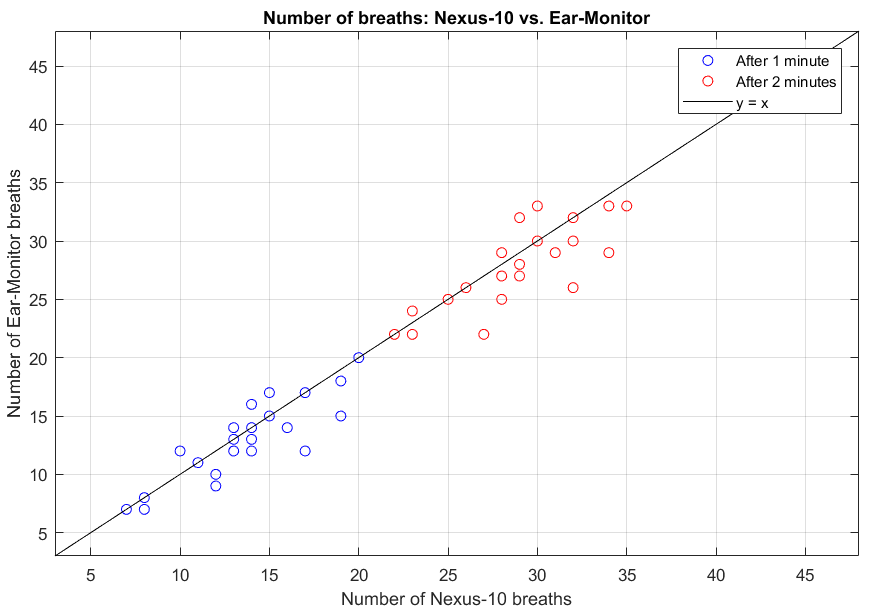
\includegraphics[width=12cm,height=7.5cm]{figs/BreathScatter.png}
   \caption{Number of breaths detected: Nexus-10 vs. Ear-Monitor (Excluding outliers)}
   \label{fig:BreathScatter}
\end{figure}

\subsection{Respiratory Rate Discussion}
The breathing exercise was included in the trial, due to the uncertainty that the RSA will be visible during normal breathing. In general, participants started breathing deeper during the breathing exercise. This resulted in a more accurate detection of breaths.

\medskip

During normal breathing, the standard deviation for the data from the breathing exercise is lower, however, the Ear-Monitor sill measured normal respiratory rate better than expected. According to the trial data (excluding the outliers), the Ear-Monitors correlates with the  benchmark device with a coefficient of 0.7604 and a p-value of zero. ICC\textsubscript{a} and ICC\textsubscript{c} indicate exceptional correlation agreement and consistency with in the 95\% confidence interval. The Ear-Monitor is able to calculate the respiratory rate of a participant breathing normally to within a mean accuracy of -0.6154 breaths per minute with a standard deviation of 1.6752 breaths per minute (11.45\% standard deviation at 15 breaths per minute). This is slightly worse, but comparable, to the 1 breath per minute accuracy from \cite{clifton2007measurement} and the 7.6\% accuracy from \cite{leonard2006fully}. This can be ascribed to the fact that they used the more advanced approach of neural networks for detecting breaths from the RSA.

\medskip

It can be seen that, on average, the Ear-Monitor detects a respiratory rate that is slightly lower (-0.5577 $\pm$1.4060 breaths per minute) than the actual rate. This means that the algorithm misses some breaths. This can be ascribed to intermittent shallower and shorter breaths that do not cause a big enough variation in heartbeat period.

\medskip

The outliers are removed to emphasize the normal results, but they are not random and provide a valuable insight into the limitations of using RSA to measure respiratory rate. It can be stated that elevated heart rates (higher than 80 bpm in this trial) reduces the magnitude of RSA  and causes the detection of false breaths. Also, if the breathing rate approaches half the heart rate (Nyquist theorem), the sampling frequency is too low and many breaths are missed by the detection algorithm. These results can be summarised by saying that respiratory rate measurement through RSA is most accurate at a combination of low heart and respiratory rates.

\section{SpO\textsubscript{2} Results}
The Ear-Monitor uses the MAX30100 pulse oximeter to measure the blood oxygen saturation of the tissue in the wall of the ear canal. One SpO\textsubscript{2} calculation is done every time the Ear-Monitor detects a heartbeat. The SureSigns VM1 from Philips is used to provide the benchmark SpO\textsubscript{2} measurement. The SureSigns VM1 samples at 1 Hz, resulting in 120 samples per recording session. As with temperature, the SpO\textsubscript{2} of a participant is assumed to stay consent over the duration of the 2-minute recording session. Therefore, the average of the SureSigns VM1 measurements and Ear-Monitor measurements are compared for each recording session.

\medskip

All trial participants are in good health and benchmark SpO\textsubscript{2} levels ranged between 96.38 and 100 \%. The measurements from the Ear-Monitor varied between 96.27 and 100\%. The mean error between the SureSigns VM1 and Ear-Monitor measurements is -0.22 $\pm$1.50\%. When plotting the Ear-Monitor and SureSigns VM1 measurements, a no significant correlation is observed. This plot can be seen in Figure \ref{fig:SpO2Scatter}.

\begin{figure}[H]
   \centering
   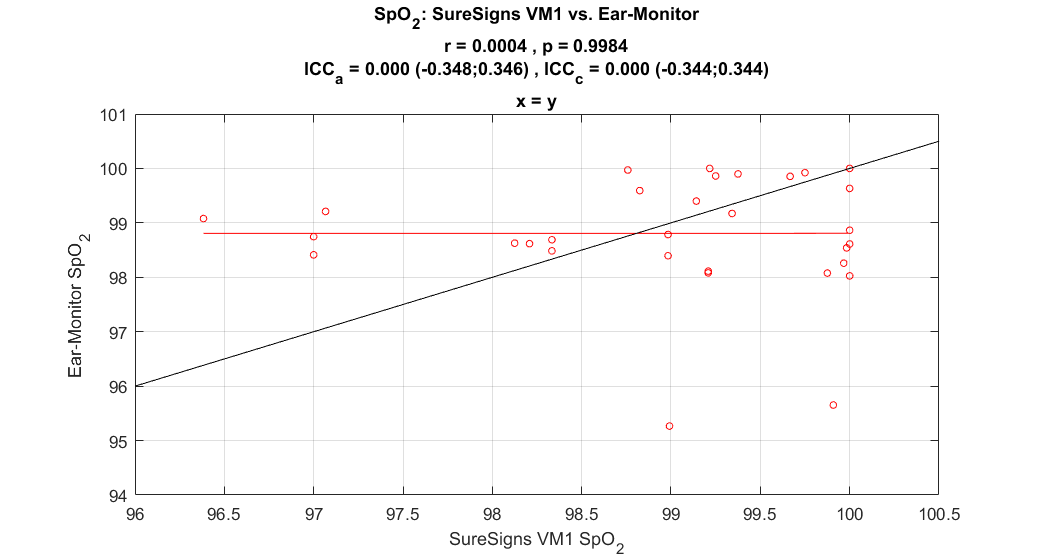
\includegraphics[width=12cm,height=7.5cm]{figs/SpO2Scatter.png}
   \caption{SpO\textsubscript{2}: SureSigns VM1 vs. Ear-Monitor}
   \label{fig:SpO2Scatter}
\end{figure}

\subsection{SpO\textsubscript{2} Results Discussion}
Analysing the trial data, it is calculated that the Ear-Monitor can measure SpO\textsubscript{2} in healthy individuals, with a mean error of -0.22 $\pm$1.50\%.

\medskip

However, because of the insignificant correlation, it can not be proven that this accuracy will continue if individuals with lower SpO\textsubscript{2} levels are monitored. An attempt was made to induce hypoxia during pilot testing by holding the breath. However, this did not cause a detectable change in SpO\textsubscript{2} measurements by the Ear-Monitor or SureSigns VM1. Clarity about the SpO\textsubscript{2} performance of the Ear-Monitor can be obtained by testing it on hypoxic patients, but testing on unhealthy individuals is not within the scope of this project. %lee2016reflectance did a test where subjects held their breath to lower SpO2, but this was not observed with the Ear-Monitor of SureSign

\medskip

The SpO\textsubscript{2} calculation method relies on the difference in the detected red and infrared light. According to the relationship found in literature, the magnitude of the infrared PPG should be higher than that of the red PPG \citep{ti2012application, strogonovsImplementing}. This can be observed in all the data recorded by the Ear-Monitor. If the wearer's SpO\textsubscript{2} decreases, the difference between the infrared and red PPGs should decrease, resulting in a higher SpO\textsubscript{2} modulation ratio (R) and, according to Equation \ref{eq:SpO2Ratio1}, a lower calculated SpO\textsubscript{2} value. This can not be observed in the trial data. The most probable reason is that the relationship is obscured by the inherent margin of error in pulse oximeters. The SpO\textsubscript{2} benchmark of the group is to constant, meaning there is not a big enough variation in SpO\textsubscript{2} among individuals to be detected by the Ear-Monitor.

\medskip

The lack of correlation within the testing range of values does not prove that the Ear-Monitor fails to measure SpO\textsubscript{2} accurately. Within the trial group, SpO\textsubscript{2} measurements all indicated participants are above the 95\% mark required for healthy adults. This is the same result as found by \cite{aziz2006pervasive}. Future testing can include hypoxic subjects and comparison with a blood gas test.

\section{Results Summary}
The statistical analysis values for the trial data is summarised in Table \ref{tab:ResultsSummary}.

\begin{table}[H]
\caption{Summary of Statistical Results}
\label{tab:ResultsSummary}
\renewcommand{\arraystretch}{1.1}
\centering
\begin{tabular}{|P{2.5cm}|P{1.4cm}|P{2cm}|P{1.1cm}|P{2.1cm}|P{2.1cm}|} 
 \hline
Vital Sign									&	Mean Error		&	Correlation coefficient	&	p-value	&	ICC\textsubscript{a}	&	ICC\textsubscript{c}\\
 \hline
Temperature Group Calibration				&	0.018  $\pm$0.513	&	0.467	&	0.014	&	0.374 (-0.01;0.66)	&	0.365 (-0.01;0.65)\\
 \hline
Temperature Intra-participant Calibration	&	-0.016 $\pm$0.290	&	0.868	&	0	&	0.875 (0.66;0.96)	&	0.868 (0.67;0.96)\\
 \hline
Heart Rate									&	0.031  $\pm$0.717	&	0.997	&	0	&	0.997 (0.99;0.99)	&	0.997 (0.99;0.99)\\
 \hline
Respiratory Rate							&	-0.558 $\pm$1.406	&	0.790	&	0	&	0.965 (0.93;0.98)	&	0.97 (0.95;0.98)\\
 \hline
SpO\textsubscript							&	-0.22  $\pm$1.50	&	0	&	0.998	&	0 (-0.35;0.35)	&	0 (-0.34;0.34)\\
 \hline
\end{tabular}
\end{table}